\documentclass[12pt]{article}
\usepackage{CJKutf8, amsmath, indentfirst, graphicx, subfigure}
\begin{document}
\begin{CJK}{UTF8}{bsmi}
\title{Mid-term Project Report}
\author{Group 8 鄭余玄、謝昀佐、陳令原}
\date{}
\maketitle
\section{團隊合作}
Mid-term project 因為我們這組決定一定要使用版本管理系統 git(圖 \ref{git})方便管理,
所以最後選擇在 GitHub 上開一個 private repo,
首先是因為這是作業,所以用 private 就不會被找到,而且如果交完作業,還可以開源讓大家來使用。

\begin{figure}[h]
  \caption{git VCS}
  \centering
  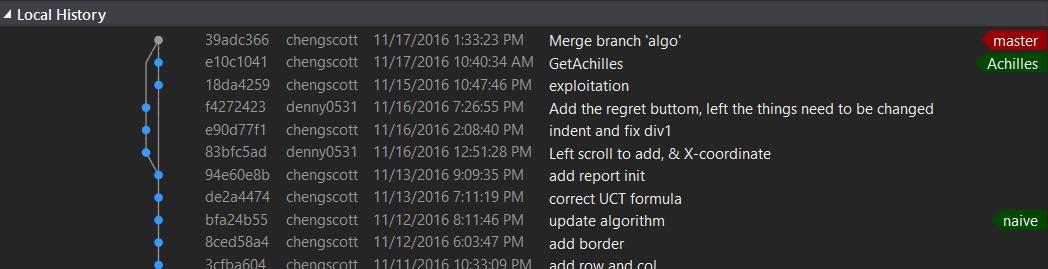
\includegraphics[width=1\textwidth]{git}
  \label{git}
\end{figure}

\section{理論運用}
蒙地卡羅樹狀搜尋(Monte Carlo Tree Search)會導致一種一維隨機漫步 \cite{MRWLTS}。
因為以前有組員寫過隨機漫步的經驗,所以稍唯有一些了解。
在考慮機率空間 $(\Omega, \mathcal{F}, P)$ 和可測空間 $(S, \Sigma)$ 之下,蒐集所有在拓樸空間 $T$ 中的 $X$ 隨機變數。
程式只會進行有限步運算,因此考慮有限機率測度 $S^k$,在合適的拓樸限制下,可以用相容的有限維機率分佈來定義這個隨機過程。

樹狀搜尋過程則是非常簡單,共分成 Selection、Simulation、Expansion 和 Backpropogation 四個階段。
這四個階段實際是如何實做的,在實驗那個段落會有說明。
在 Simulation 階段,我們參考威脅空間搜尋 \cite{threatspaces} 的想法,要產生一場勝利的棋局充分必要條件是產生兩個以上的威脅。
這其實十分直觀,而該篇論文也對威脅稍做分類整理,我也整理出類似的公式:
$\phi$ stands for AI($\psi$) or Opponent($\varphi$)

\[\begin{split}
\phi(4) &= \phi(4, 1) + \phi(4, 2)\\
\phi(3, 1)&\cong\phi(4, 2)\\
\phi(2, 1)&\cong\phi(3, 2)
\end{split}\]
$\phi$ wins if $\phi(\geq 5)>0$; otherwise, find $\arg\max\{\phi(4, 1),  [\phi(3, 1)] +  [\phi(3, 1)]\}$.

此外,UCT-child 則是使用常見公式 $\arg\max\{\frac{w_i}{n_i}+\sqrt\frac{2\log\sum_i{n_i}}{n_i}\}$,原因在實驗也有詳細說明。

\begin{figure*}[h]
  \caption{mcts.cpp: Line 98}
  \centering
  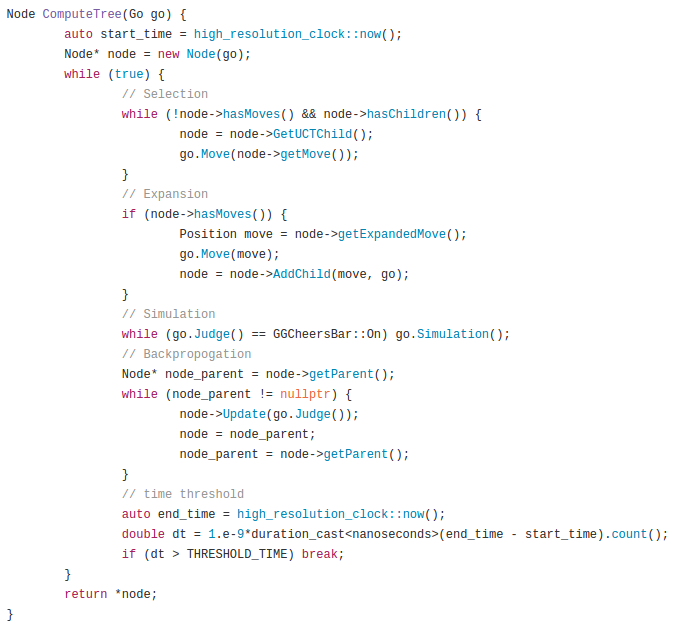
\includegraphics[width=.8\textwidth]{tree}
\end{figure*}

\section{實做過程}
MCTS 會運用到大量的節點展開,因此我們選用 C/C++ 來實做核心功能,目的是為了透過越底層的指標操作,來減低計算複雜度的常數。
而棋盤顯示部份則是用 HTML5 和 JavaScript 來完成,中間希望藉由 socket 來建立連線,就不用重複計算展開的節點。
當初構想是可以讓核心的 C 程式遠端跑在效能更到的電腦上,不過因為後來老師宣佈不能連上網路,所以也就做罷。
這套系統架構的規劃是非常有彈性的,假如今天有新的棋盤外觀模組,則只需要抽換前端即可,核心判斷程式完全照常運作。
此外,若考慮人和人或 AI 之間的連線,之需要針對中間層 socket 做適當的改變,其他部份一樣是照舊。
而且在這規劃之下,組員之間分工可以較明確。

主程式整體結構上,雖然要求效能,但是 Donald Knuth 說過,過早的優化是邪惡的 \cite{Knuth},因此開發時主要是避免一些 overhead 和降低演算法複雜度。
所有物件皆有良好的封裝,也有參考一些設計模式,像是 Strategy 模式等等,以及盡量去遵守 S.O.L.I.D. 原則。
所有程式碼,像是程式變數命名、物件區塊順序等細節皆有按照 Google Coding Style \cite{gcs},讓我們這組開發上有一致的規範。

此外,MCTS 也十分著重隨機性,從前述的理論就可以略知一二。
但是 C/C++ 所提供亂數函式庫是惡名昭彰的不隨機,因此特別選用了 C++11 提供的 mersenne twister engine(mt19937)去做隨機分佈。

\section{實驗}
在開始實做這份專案之前,我們參考了許多篇論文。
但是許多篇論文總是聲稱某些參數被控制的情況下,MCTS 則可以收斂,但至於是否能有效的收斂則是一個問題。
(因為題目規定 10 秒內完成計算,但是參考許多案例,要得到一般好的結果,通常需要約是四十秒左右)
當然,計算時間及複雜度往往是依問題的限制條件多寡而有所不同 \cite{SVMCTS}。
因此就實際而言,許多參數都只能藉由不斷猜測、嘗試和實驗而得到的。
所以專案大部分的時間,都是在對常數和細節微調。

經過幾次的實驗之後,蒙地卡羅的搜尋樹通常會長成圖\ref{search},但是這種樹非常容易形成混沌系統\cite{CHAOS}。
一旦變成混度系統,因為成長參數會太大,而且導致非常容易崩塌(MCTS 的隨機性更是會突顯這件事)。
實驗上則是更困難,因為一旦初始條件微調,結果就會有極大的擾動。
\begin{figure*}[h]
  \caption{搜尋樹}
  \centering
  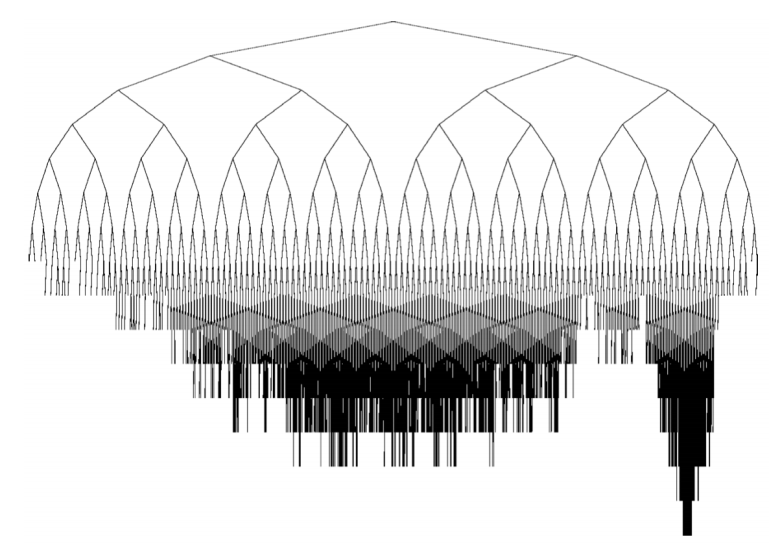
\includegraphics[width=.5\textwidth]{search}
  \label{search}
\end{figure*}


MCTS 主要困難的地方是在權衡 exploration 和 exploitation 的比例。
如果只仰賴隨機性,則程式需要展開更多的節點,以時間換取空間。
但是因為限時 10 秒,所以勢必要加入更多 exploitation 的成份。
原本有考慮是否要針對現有的「必勝」棋譜去做匹配,考慮複雜度的情況,是可以負荷的,
但是當我們完成「naive」版本的 MCTS 時,我們就知道不需要做了。
參考圖 \ref{intelligent} ,如果對照一下常見棋譜,到第八步以前是所謂的「溪月」開局\cite{Keigetsu}。
也就是說其實光是只靠 exploration 就可以計算出良好的位置,如果在加上更多 domain knowledge 的 exploitation,那更是如虎添翼。
因此後來就不打算去匹配棋譜。

\begin{figure*}
  \caption{前期為「溪月」開局法}
  \centering
  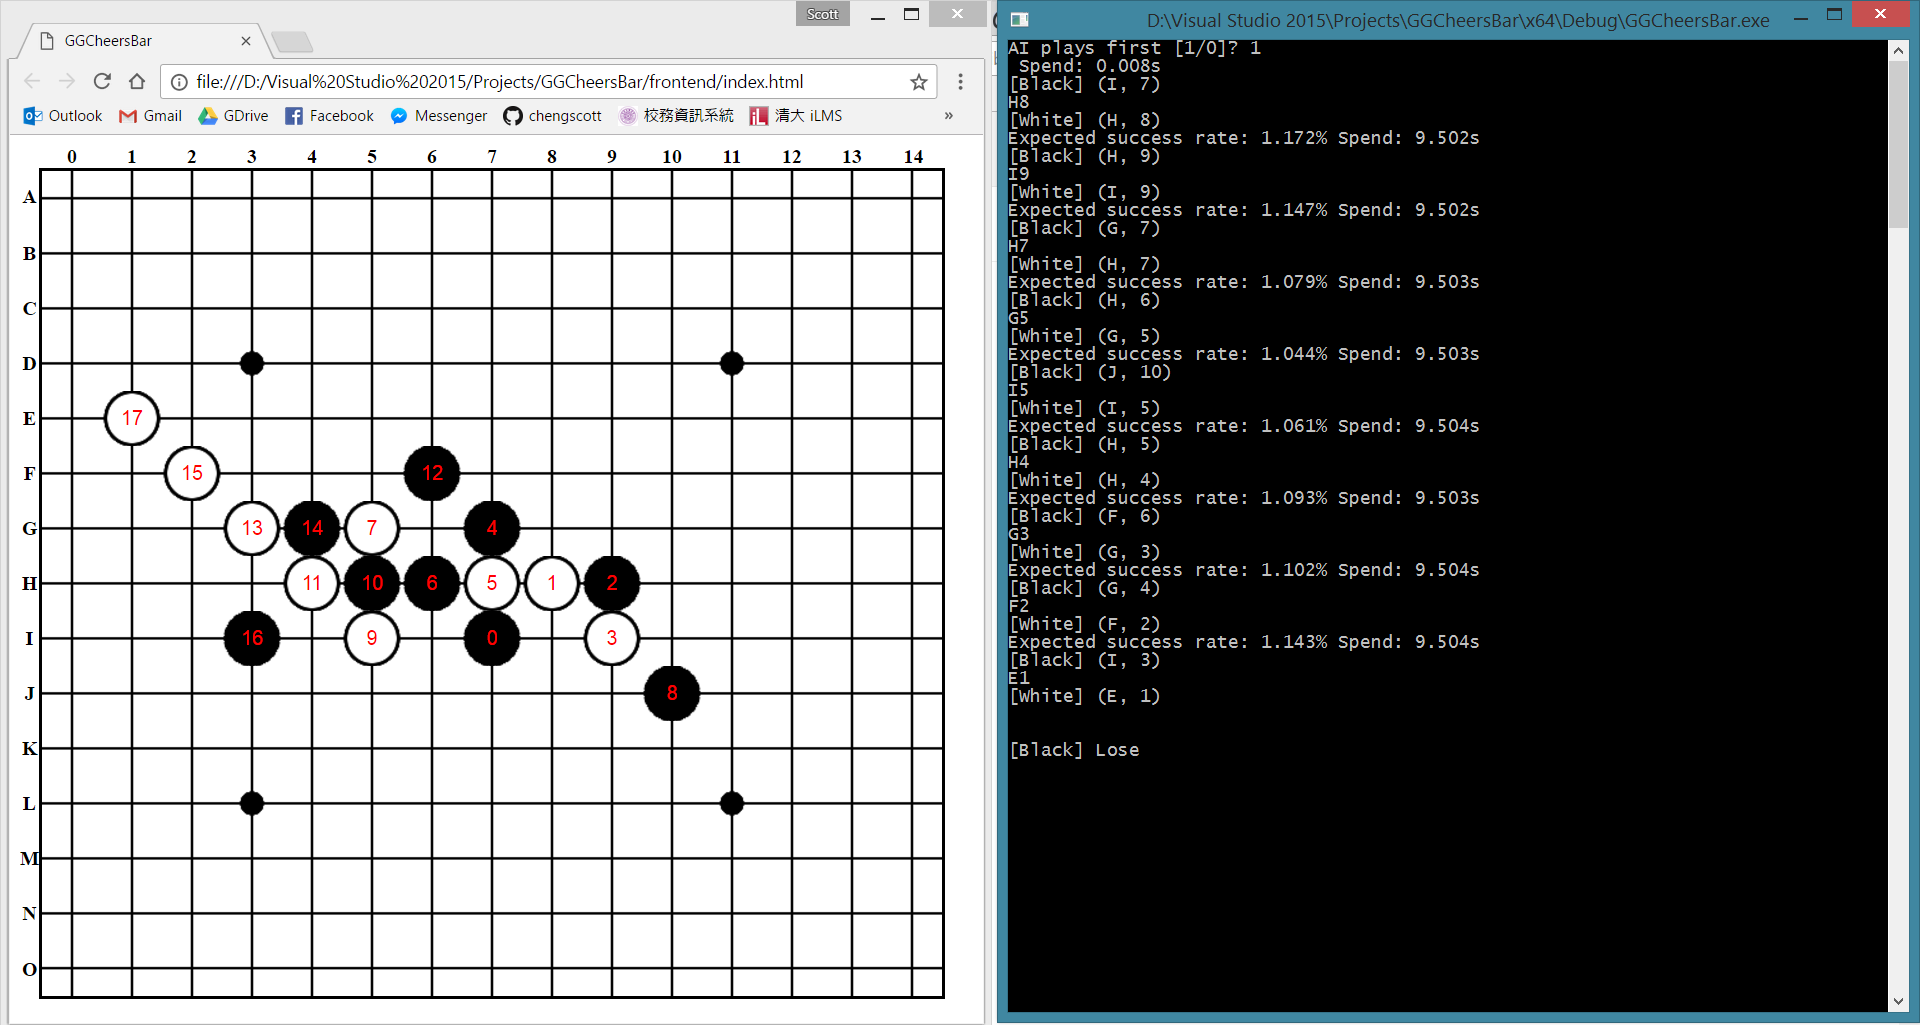
\includegraphics[width=1\textwidth]{intelligent}
  \label{intelligent}
\end{figure*}

但是當 exploitation 成份越來越多時,情況就會變得如圖 \ref{exploitation}。
也就是說程式過度著重策略,而忽略了探索導致出現非常保守的局面。
而且我們還發現,若是在 Simulation 階段使用 exploitation,則節點展開越深,exploitation 影響力越低。
從直觀來說,很顯然展開越多,則探索(exploration)越多;
就計算而言,展開越深則策略的權重影響更小,因為很多權重小的和可能大過一個大權重的。

\begin{figure*}[h]
  \caption{過多 exploitation}
  \centering
  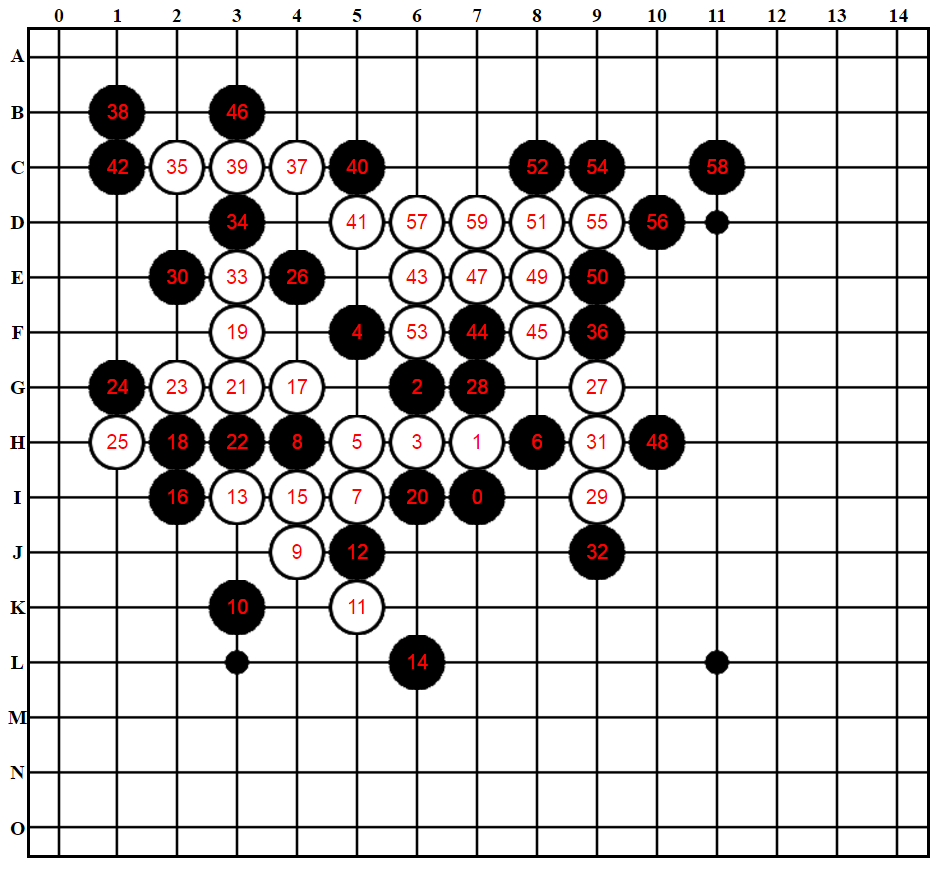
\includegraphics[width=.6\textwidth]{defense}
  \label{exploitation}
\end{figure*}

再不斷調整策略以後,我們最終的版本是在 Selection 部份加強 exploitation,而 Simulation 則側重 exploration,讓 MCTS 有更多探索的可能性。
最終的這個版本我們則稱它「Achilles」,因為他的策略就如同阿基里斯的後腳跟一樣致命。

最後我們拿同一支 AI 對弈,結果如圖 \ref{equi}。
因為繳交期限的緣故,所以最後沒有再做更深入的探討,不過我們猜測那是納許均衡的結果,或許遊戲已經達到一種平衡。

\begin{figure*}[h]
  \caption{兩支 AI 均衡態}
  \centering
  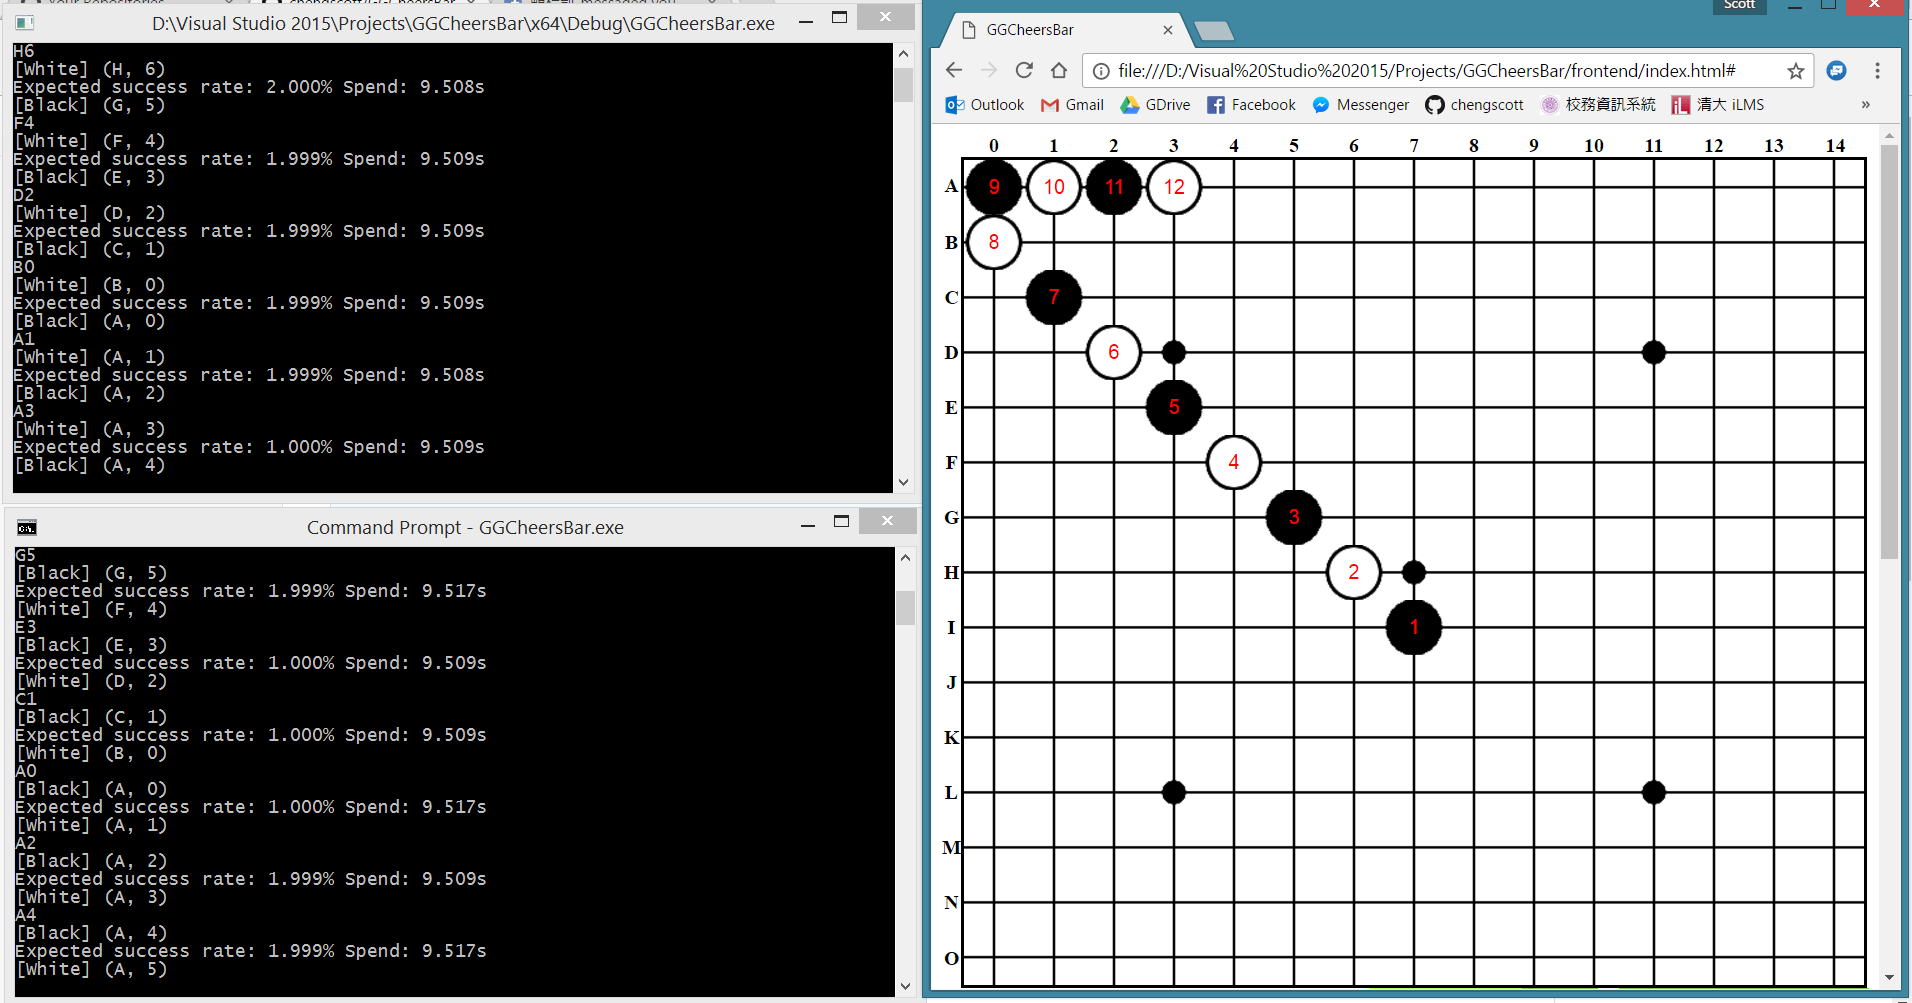
\includegraphics[width=1\textwidth]{equilibrium}
  \label{equi}
\end{figure*}

\section{效能調校}
除了程式實做驗證理論以外,我們還有對演算法做效能評估(圖 \ref{performance})。
MCTS 四個主要階段最消耗資源的是 Backpropogation 中的計算 UCT,佔了將近九成的資源。
原本打算使用一維線段樹來維護操作,降低時間複雜度,但是因為組員不熟悉此資料結構而作罷。
此外,每當程式在計算時,非常仰賴 CPU 運算資源。
但是組員們因為技術上的困難,對於多線程編程並不是很熟悉,因此就只能針對實做細節調校。

\begin{figure*}
  \caption{效能瓶頸}
  \centering
  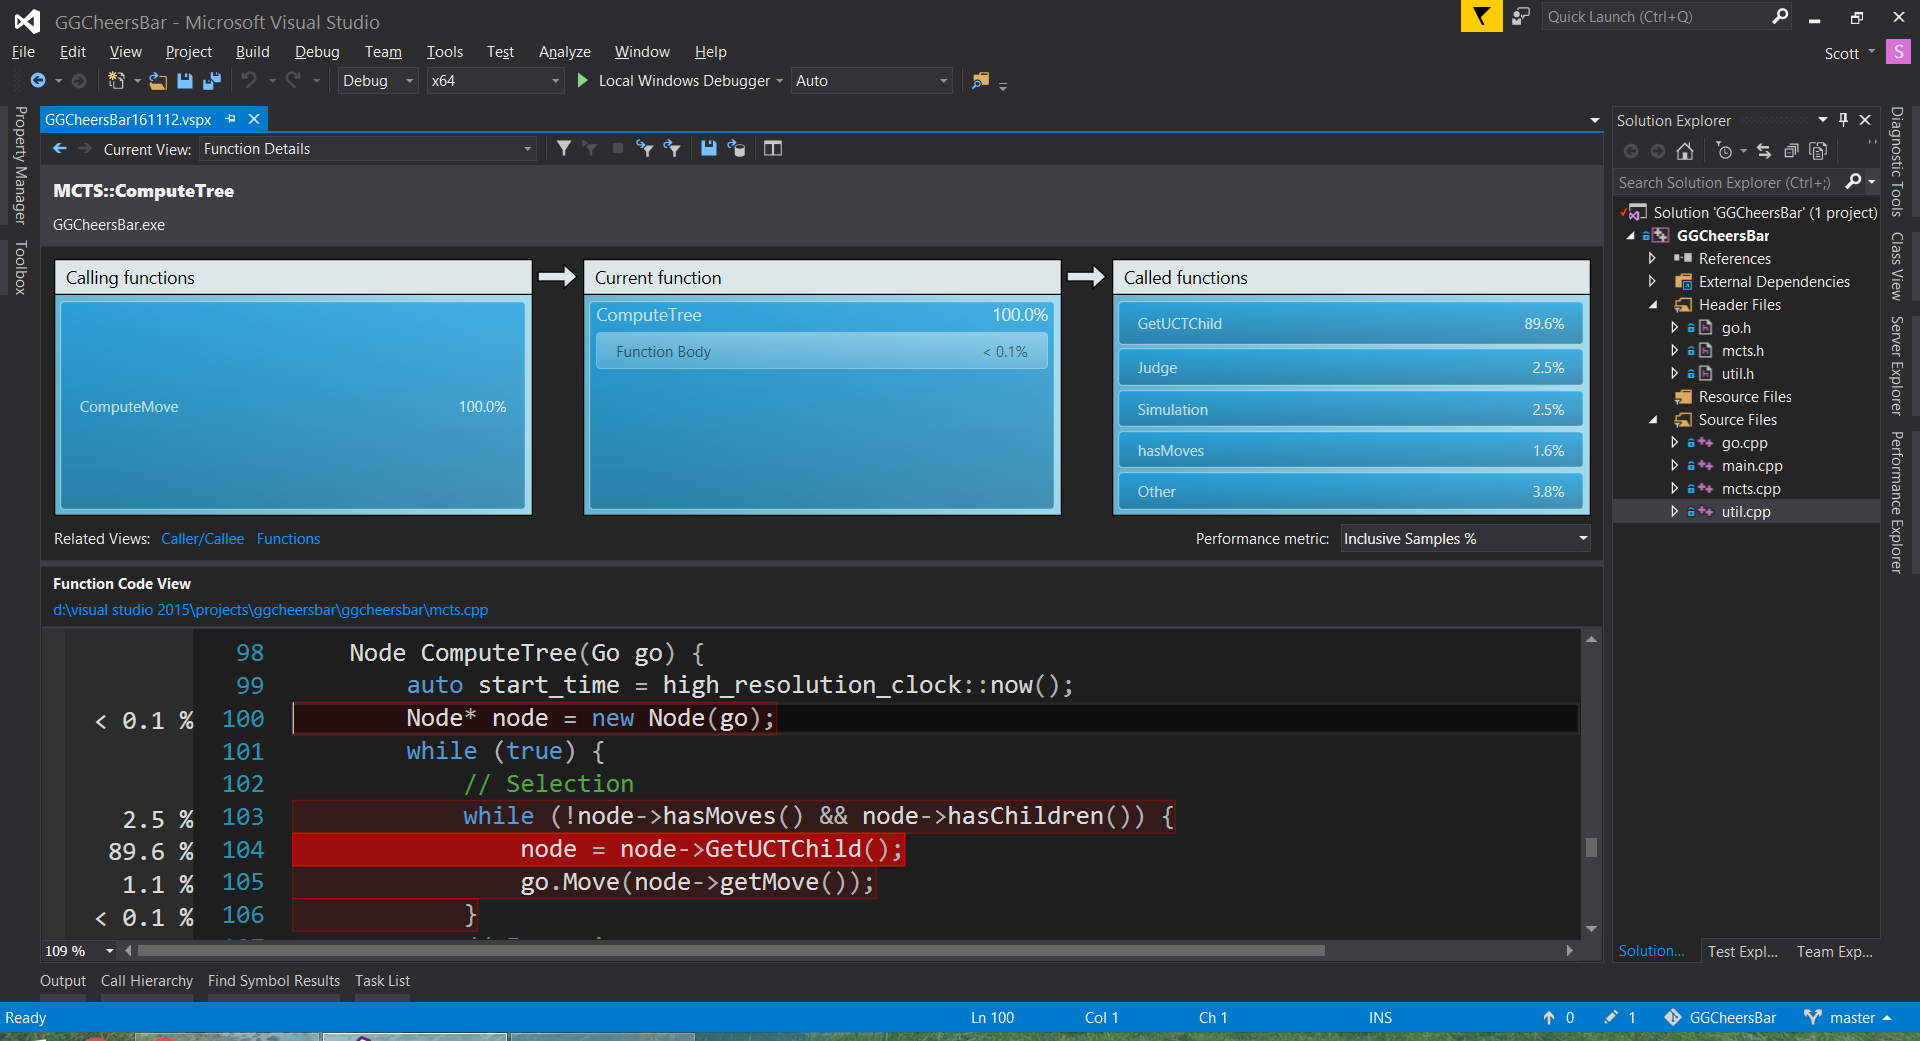
\includegraphics[width=1.2\textwidth]{performance}
  \label{performance}
\end{figure*}

\bibliographystyle{IEEEtran}
\bibliography{./refs}
\end{CJK}
\end{document}
